\documentclass[tikz]{standalone}
\usepackage{amsmath,amssymb}
\usepackage{tikz}
\usetikzlibrary{
	shapes,
	snakes,
	calc,
	decorations,
	decorations.markings,
	decorations.text,
	decorations.pathreplacing}
	
\begin{document}
\begin{tikzpicture}[scale=1,auto,every text node part/.style={align=center}]
  \definecolor{darkred}{rgb}{0.4,0,0}
  \definecolor{darkblue}{rgb}{0,0,0.4}
  \definecolor{darkgreen}{rgb}{0,0.4,0}

%%   \node[darkgreen] (More) at (2,0) {
%%     \begin{tikzpicture}
%%       \node (M0) at (0,3.6) {More(one hundred one, fifty two)\\0};
%%       
%%       \node (LB1) at (-8,2.4) {LargerBase(hundred, $\varnothing$).\\1};
%%       \node (P2) at (-9,1.2) {PrevBase(hundred, $\varnothing$).\\};
%% 
%%       \node (N1) at (-2,2.4) {Number(one hundred one)\\2};
%%     
%%       \node (Nu1) at (5,2.4) {Number(fifty two)\\3};
%%   
%%       \node (P1) at (-5,1.2) {Prefix(one, hundred)\\4};
%%       \node (O2) at (-6.5,0) {Ones(one).\\};
%%       
%%       \node (S1) at (0,1.2) {Suffix(hundred, one)\\5};
%%       \node (LB2) at (-3,0) {LargerBase(hundred, $\varnothing$).\\6};
%%       \node (P3) at (-3,-1.2) {PrevBase(hundred, $\varnothing$).\\};
%%       \node (N2) at (1.5,0) {Number(one)\\7};
%%       \node (Pr3) at (3,-1.2) {Suffix($\varnothing$, $\varnothing$).\\};
%%       \node (Su3) at (0,-1.2) {Prefix(one, $\varnothing$)\\8};
%%       \node (O4) at (-1.5,-2.4) {Ones(one).\\};
%%       
%%       \node (Pr1) at (9.5,1.2) {Suffix($\varnothing$, $\varnothing$).\\};
%% 
%%       \node (Su1) at (5.5,1.2) {Prefix(fifty two, $\varnothing$)\\9};
%%       \node (D2) at (5,0) {Decades(fifty).\\};
%%       \node (On2) at (7.5,0) {Ones(two).\\};
%%             
%%       \draw [<-] (M0)     to (LB1);
%%       \draw [<-] (M0)     to (N1);
%%       \draw [<-] (M0)     to (Nu1);
%%       \draw [<-] (N1)     to (P1);
%%       \draw [<-] (N1)     to (S1);
%%       \draw [<-] (Nu1)     to (Pr1);
%%       \draw [<-] (Nu1)     to (Su1);
%%       \draw [<-] (LB1)    to (P2);
%%       \draw [<-] (P1)     to (O2);
%%       \draw [<-] (S1)     to (LB2);
%%       \draw [<-] (S1)     to (N2);
%%       \draw [<-] (LB2)     to (P3);
%%       \draw [<-] (N2)     to (Pr3);
%%       \draw [<-] (N2)     to (Su3);
%%       \draw [<-] (Su3)     to (O4);
%%       \draw [<-] (Su1)     to (D2);
%%       \draw [<-] (Su1)    to (On2);
%%   \end{tikzpicture}};

  \node[anchor=north,darkblue] (Number) at (-7,0) {
  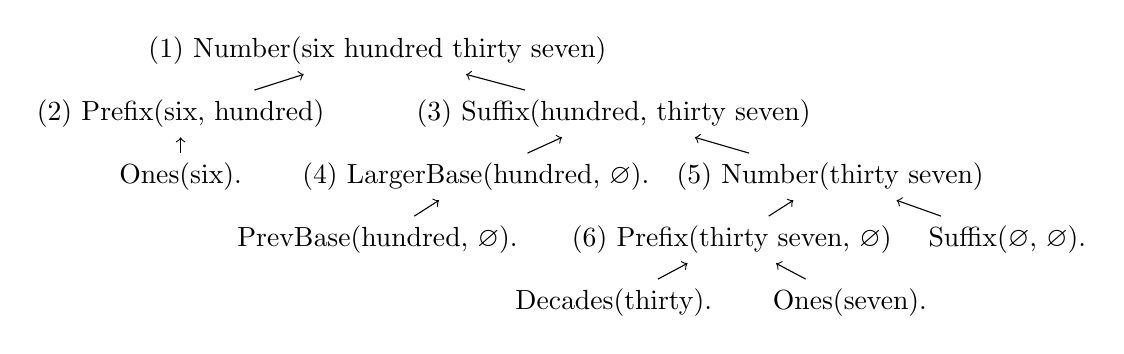
\begin{tikzpicture}
    \node (N0) at (0,1.6) {(1) Number(six hundred thirty seven)};
    \node (P1) at (-2.5,.8) {(2) Prefix(six, hundred)};
    \node (S1) at (3,.8) {(3) Suffix(hundred, thirty seven)};
    \node (O2) at (-2.5,0) {Ones(six).};
    \node (LB2) at (1.25,0) {(4) LargerBase(hundred, $\varnothing$).};
    \node (N2) at (5.75,0) {(5) Number(thirty seven)};
    \node (P3) at (8,-.8) {Suffix($\varnothing$, $\varnothing$).};
    \node (S3) at (4.5,-.8) {(6) Prefix(thirty seven, $\varnothing$)};
    \node (D3) at (3.,-1.6) {Decades(thirty).};
    \node (O3) at (6.,-1.6) {Ones(seven).};
    \node (PB3) at (0,-.8) {PrevBase(hundred, $\varnothing$).};
    
    \draw [<-] (N0) to (P1);
    \draw [<-] (N0) to (S1);
    \draw [<-] (P1) to (O2);
    \draw [<-] (S1) to (LB2);
    \draw [<-] (LB2) to (PB3);
    \draw [<-] (S1) to (N2);
    \draw [<-] (N2) to (P3);
    \draw [<-] (N2) to (S3);
    \draw [<-] (S3) to (D3);
    \draw [<-] (S3) to (O3);
  \end{tikzpicture}};
  


  \node[anchor=north,darkred] (Succ) at (6,0) {
    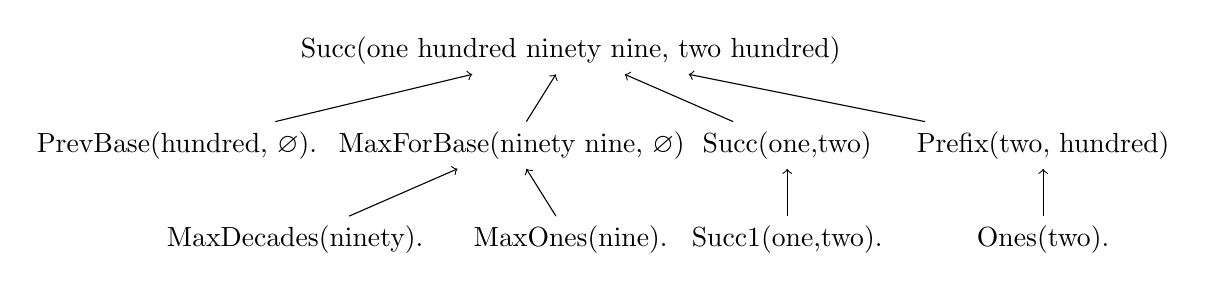
\begin{tikzpicture}
      \node (S0) at (2,2.4) {Succ(one hundred ninety nine, two hundred)};
      
      \node (PB1) at (-3,1.2) {PrevBase(hundred, $\varnothing$).};

      \node (MFB1) at (1.25,1.2) {MaxForBase(ninety nine, $\varnothing$)};
      \node (MD2) at (-1.5,0) {MaxDecades(ninety).};
      \node (MO2) at (2,0) {MaxOnes(nine).};

      \node (S1) at (4.75,1.2) {Succ(one,two)};
      \node (SO2) at (4.75,0) {Succ1(one,two).};

      \node (P1) at (8,1.2) {Prefix(two, hundred)};
      \node (O2) at (8,0) {Ones(two).};
      
      \draw [<-] (S0)     to (MFB1);
      \draw [<-] (S0)     to (PB1);
      \draw [<-] (S0)     to (P1);
      \draw [<-] (S0)     to (S1);
      \draw [<-] (MFB1)   to (MD2);
      \draw [<-] (MFB1)   to (MO2);
      \draw [<-] (S1)     to (SO2);
      \draw [<-] (P1)     to (O2);
  \end{tikzpicture}};
\end{tikzpicture}
\end{document}
